% What kind of text document should we build
\documentclass[noprint]{uit-thesis}


% Include packages we need for different features (the less, the better)
\usepackage{hyperref}
\hypersetup{
    colorlinks=true,
    linkcolor=blue,
    filecolor=magenta,      
    urlcolor=cyan,
    citecolor=blue,
}
\usepackage{graphicx,wrapfig,lipsum}
\usepackage{multicol}
\usepackage{nameref}
\usepackage{makecell}




% Math
\usepackage{amsmath}

% Clever cross-referencing
\usepackage{cleveref}

% Algorithms
\usepackage{algorithm}
\usepackage{algpseudocode}
\algdef{SE}[DOWHILE]{Do}{doWhile}{\algorithmicdo}[1]{\algorithmicwhile\ #1}%

% Tikz
\RequirePackage{tikz}
\usetikzlibrary{arrows,shapes,calc,through,intersections,decorations.markings,positioning}
\usepackage{tikz}
\usetikzlibrary{shapes, arrows.meta, positioning}

\tikzstyle{every picture}+=[remember picture]

\RequirePackage{pgfplots}
\RequirePackage{pgfplotstable}

% Better bibliography 
\usepackage[round]{natbib}





\begin{document}

%:-------------------------- Frontpage ------------------------
\title{Hill ascent confidence model and simulator for trailer trucks}
\subtitle{ }% Note: this is optional, and may be commented out
\author{Tanja Emilie Henriksen}
\thesisfaculty{Faculty of Engineering Science and Technology \\ Department of Computer Science and Computational Engineering}
\thesisprogramme{DTE-3900 Master's thesis in Applied Computer Science May 2022}

\maketitle

%:-------------------------- Frontmatter -----------------------
\frontmatter

\begin{abstract}
This master thesis reports on the research of simulating hill ascensions on winter roads. By utilizing Python and Excel a simple prototype simulation was created. This simulation shows the velocity changes during the ascension, with different variables such as: initial velocity, gear, weight distribution, environment etc. The variables used are mostly based on real life measurements, with a few exceptions where educated guesses where taken. 
\par
The results of the simulation shows clearly how the different variables impact the simulation. These results reflect the expected outcome and statements from other research papers. Additionally these results also proves the hypothesis: It is not only the physical aspects of a hill ascension that needs to be taken into consideration, but also how the driver is driving. Especially when it comes to what gear is being used and the impact of a gear change during the ascension. Further validation of the accuracy cannot be taken before proper experiments and potential tuning are completed.

\end{abstract}

\begin{acknowledgement}
I would first of all thank my supervisor Rune Dalmo for all the help and support during this thesis. Our frequent “sanity checks” have helped me improve my work and keeping me motivated. This thesis would never be finished without you. 
\par
I would also give a huge thanks to my classmates for the tremendous help during the master course. Without you helping and sharing your knowledge, I would never be able even start on my thesis. I will truly miss our celebratory/motivating cake Fridays. 
\end{acknowledgement}

\tableofcontents
\listoffigures
\listoftables

%:-------------------------- Mainmatter -----------------------
\mainmatter




\chapter{Introduction}
Road friction is crucial to traffic safety. Winter roads can be challenging since the conditions may change rapidly. One of the most abrupt factors for people and businesses in the Arctic region is the closing of main roads due to trailer trucks in need of rescue. 
\par 
Most of the previous works on road friction and its correlation with traffic safety has been focusing on the risk of accidents ~\citep{Friction}. But closing of a road reasoned by a trailer truck needing rescue because it was unable to ascent a hill causes cascading problems for the community. For example, it affects the abilities to clean the roads for snow, salting or sanding, and assisting for rescues. This in turn makes the roads less safe and thus increases the risk of accidents.
\par
A simulation could help predict the chances of a trailer truck being unable to ascent a hill. This could potentially reduce the yearly resources needed to rescue these trailer trucks tremendously. 

\section{Relevance}
It is not an uncommon occurrence that trailers are unable to ascent hills and stops traffic. The local newspaper Fremover, have documented several rescue cases involving trailers unable to ascent hills due to winter roads. ~\citep{Treldal} and ~\citep{Taraldsvikbakken} is both such cases. A thesis like this can help lay the groundwork and potentially help create a fully functional simulation. This simulation could predict whenever you as a truck driver may be able to ascent with your current equipment or not. With further research it could even help tell the drivers if they need to put on chains or change their driving style. 



\section{Problem description}
The main purpose of this thesis is to research the possibility of creating a realistic simulation of trailer trucks trying to ascent a hill. This research includes: 
\begin{itemize}
\setlength\itemsep{-0.3cm}
\item Create a model and evaluate its accuracy.
\item Show the effects of adjusting certain parameters, such as initial velocity, friction, etc. 
\item Debate to which extent does the trade-off between complexity and simplicity affect the uncertainty of the model is also an important aspect of the research. For example, is a simplified model still useful and/or relevant?
\end{itemize}


\section{Inputs and variable parameters}
There are several variables needed to be taken into consideration when creating the simulation. The road condition, the truck model and hill steepness are some of the basic variables we need for a working simulation. The main factors regarding variables are the complexity and realism of the simulation. When choosing between complex and simplistic variables the trade-off between accuracy and runtime need to be taken into consideration. A complex and correct friction calculation can give a more realistic result, but a demo might have such a long runtime that it is practically useless. 

\subsection{Accuracy}
The accuracy of the simulation is heavily reliant on how good the compensation for the inaccuracy and range of the parameters are. Both the friction coefficient and the trailers acceleration are parameters with a potentially high inaccuracy, as well as a great influence on the end result. 

\section{Friction} 
As mentioned earlier, the friction estimation and calculation are important aspects of the simulation. Where even a slight change of the friction coefficient can change the result tremendously. There are two main approaches for friction estimation, model-based and experiment-based approach ~\citep{frictionEstimation}. 


\subsection{Model-based approach}
Model-based approaches contains all the methods using mathematical or dynamical models to estimate the friction. The lack of requirements for any specialized sensor and the repeatability of the results in most cases, makes the model-based approach more used than the experiment-based approach. There are several parameters needed to calculate pavement friction, table \ref{tab:fricFactors} gives an overview over these needed parameters and factors. 

%Table of factors
\begin{table}[H]
\center
\begin{tabular}{|p{0.5\linewidth} | p{0.5\linewidth} |} 

 \hline
 \textbf{\large Pavement Surface
 Characteristics}
& \textbf{\large Tire Properties} \\ [0.5ex] 
 \hline

\begin{itemize}
 \item Microtexture 
 \item Macrotexture
 \item Megatexture
 \item Unevenness
 \item Material properties
 \item Temperature
\end{itemize}

& \begin{itemize}
 \item Foot Print
 \item Tread design and condition
 \item Rubber composition and hardness
 \item Inflation pressure
 \item Load
 \item Temperature 
\end{itemize} \\ 

\hline \hline
\textbf{\large Vehicle Operating Parameters} 
& \textbf{\large Environment} \\ [0.5ex] 
\hline

\begin{itemize}
 \item Slip speed
 \begin{itemize}
  \item Vehicle speed
  \item Braking action
 \end{itemize}
 \item Driving maneuver
 \begin{itemize}
  \item Turning
  \item Overtaking
 \end{itemize}
\end{itemize}

& 
\begin{itemize}
 \item Climate
 \begin{itemize}
  \item Wind
  \item Temperature
  \item Water (rainfall, condensation)
  \item Snow and Ice
 \end{itemize}
 \item Contaminants 
 \begin{itemize}
  \item Anti-skid material (salt, sand)
  \item Dirt, mud, debris
 \end{itemize}
\end{itemize} \\ 

\hline

\end{tabular}
\caption{Factors affecting available pavement friction ~\citep{Friction}.}
\label{tab:fricFactors}
\end{table}

%END of Table of factors




\subsection{Experiment-based approach}
Figure~\ref{fig:FlowChartExperiment} demonstrates the main philosophy behind experiment-based approach. The majority of experiment-based methods used sensors for measuring the friction-related parameters, and then try to correlate these parameters to tire-road friction. 
\par
\begin{figure} [H]
\centering
	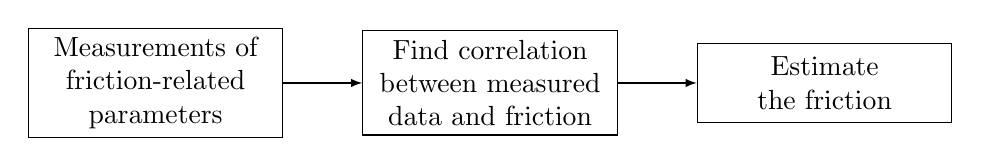
\begin{tikzpicture}
	% draw rectangle node
	\node[draw,
	minimum width=2cm,
	minimum height=1cm,
	text width=3cm,
	text centered] (block1) {
	Measurements of friction-related parameters
	};
	\node[draw,
	minimum width=2cm,
	minimum height=1cm,
	right=of block1,
	text width=3cm,
	text centered] (block2) {
	Find correlation between measured data and friction
	};
	\node[draw,
	minimum width=2cm,
	minimum height=1cm,
	right=of block2,
	text width=3cm,
	text centered] (block3) {
	Estimate the friction
	};
	% Arrows
	\draw[-latex] (block1) edge (block2)
	(block2) edge (block3);
	\end{tikzpicture}

\caption{Experiment-based flowchart diagram.}
\label{fig:FlowChartExperiment}
\end{figure}


There are three main types of sensor types used for experiment-based approaches, optical sensors and cameras, acoustic sensor, and tire tread sensors. The optical sensors and cameras are used for detecting surface properties related to friction. The acoustic sensors are used for classifying the road surface type and condition. These sensors can determine whenever the road is wet dry, asphalt, concrete, etc. based on the tire noise. The tire tread sensors are used to monitor the interaction between the tire and the road, estimating the deflection of tread elements inside the contact patch. 



\section{Truck}
There are certain choices and limitations needed to be taken into consideration regarding the truck used for the model and its variables. The first limitation is choosing one specific truck. Scania was in 2021 Norway’s most bought truck brand ~\citep{2021Truck}. All of their trucks are highly customizable so even trucks of the same model can have differences ~\citep{Scania}. Scania’s R580 models are often seen on roads and on online listings. It is therefore decided to use a Scania R580 with both 6x2 and 6x4 drive and a Euro 6 engine for the confidence model and simulation. The needed specifications are taken from Scania’s spec sheets R 520 LA6x4ESZ Euro 6 ~\citep{R520} and R 580 6X4 PRIME MOVER Chassis Specification ~\citep{R580}.
\par
\begin{figure}[H]
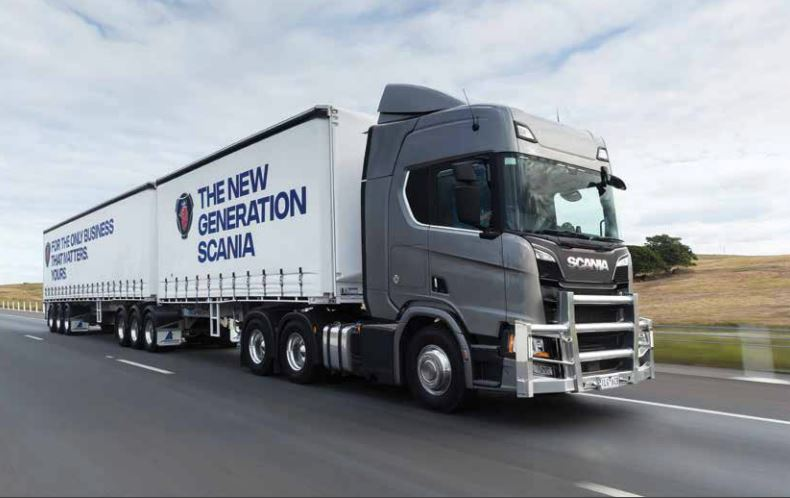
\includegraphics[width=\textwidth]{./photo/R580.JPG}
\caption{Photo of a Scania R580 6x4 ~\citep{R580}}
\label{fig:R580}
\end{figure}

\par
Experienced truck drivers have several tricks to rise the chance of ascending, such as temporarily increasing the pressure on the driving axles. These techniques are not taken into consideration when generating the simulation. 
\par
When the force delivered to the tyre tread exceeds that of available tread-to-surface friction and one or more tyres loose traction, a wheelspin occurs. Wheelspins greatly reduces the chances of successfully ascending the hill. For this project it is assumed that the driver have “perfect” control on the accelerator pedal resulting in no wheelspins. 

\subsection{Gear change}
The R580 is an older model so the gearing might be a bit slower and noticeable than on newer trucks. It is therefore decided that the truck is using approximately two seconds to change gear. There are also no strict rules when it comes to speed and gears, it is therefore taken an educated guess on what gears might be suitable for different speeds. 


%Method
\chapter{Method}
For this thesis a theoretical approach was chosen to create the prototype simulations, also called models. Since these models are theoretical, they need to be validated through experiments. The method section is therefore mainly divided into \nameref{models}, \nameref{validation} and \nameref{implementation}.
\par
To gain insight and knowledge of hill ascension and especially why they fail, we consulted with the experienced tow truck driver Trond Olsen owner of Narviking AS ~\citep{narviking}. This consulting meeting lead to a hypothesis that it is not only the physical aspects of the model, such as friction, mass, speed etc, that needs to be taken into consideration, but also how the driver is driving. It was expected that what gear is being used and if the gear is changed during the ascension, would have a big impact on the successfulness of the hill ascension.
\par
An experiment-based approach was chosen for the estimation of friction coefficient, due to the complexity and the amount of parameters needed to get an acceptable calculated friction coefficient. The measured values are collected from both an official report from the Norwegian Public Roads Administration ~\citep{vegvesene}, and earlier experiments from UiT campus Narvik.



\section{Models}
\label{models}
There are two models made, “The basic driving simulation” (BD sim) and “The forced gearing simulation” (FG sim). The models are based on a state system to easier divide and explain the processes. There are three states in this system, Force check, Speed reduction and Speed gain. 
\par
The basic driving simulation starts in the Force check state and goes either to Speed reduction or Speed gain depending on the sum of forces, then returns to Force check as seen in figure \ref{fig:StateDiagram}. This means that the truck maintains the same gear throughout the simulation. 

\begin{figure} [H]
\centering
	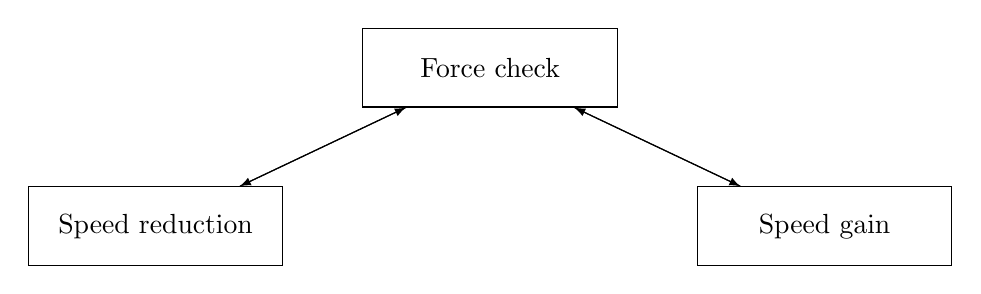
\begin{tikzpicture}
	% draw rectangle node
	\node[draw,
	minimum width=2cm,
	minimum height=1cm,
	text width=3cm,
	text centered] (block1) {
	Force check
	};
	\node[draw,
	minimum width=2cm,
	minimum height=1cm,
	below right=of block1,
	text width=3cm,
	text centered] (block2) {
	Speed gain
	};
	\node[draw,
	minimum width=2cm,
	minimum height=1cm,
	below left=of block1,
	text width=3cm,
	text centered] (block3) {
	Speed reduction
	};
	% Arrows
	\draw[-latex] (block1) edge (block2)
	(block1) edge (block3)
	(block2) edge (block1)
	(block3) edge (block1);
	\end{tikzpicture}

\caption{State flowchart diagram.}
\label{fig:StateDiagram}
\end{figure}

The forced gearing simulation is built upon the basic driving simulation, but after driving half way up the hill the truck is forced to gear down one gear. As mentioned earlier the truck uses two seconds to change gear, during this time the truck enters speed reduction without any force pulling it forward. This is achieved by setting the gearing ratio to zero before entering the Force check and Speed reduction state.


Table \ref{tab:variables} shows some of the variables used in the formulas for the trailer truck models. The distance until current state ends ($DS$) is the distance until an environmental parameter, such as the friction or hill steepness changes. 


%Table of variables
\renewcommand{\arraystretch}{1.25}
\begin{table}[H]
\center
\begin{tabular}{|p{0.49\linewidth} | p{0.49\linewidth}|} 

 \hline
\multicolumn{2}{|c|}{Variables} \\
 \hline 
m[$kg$] & Mass \\
g[$m/s^2$] & Gravitational constant $= 9,81$ \\
AR & Weight distribution ratio over drive axle \\
GR & Gear ratio \\
DR & Differential ratio \\
TE & Transmission efficiency \\
Wr[$m$] & Wheel radius \\
ET[Nm] & Engine torque \\
D[m] & Displacement \\
DS[m] &  Distance until current state ends \\
DZ[m] & Distance until the speed is reduced to zero \\
$V_{limit} [m/s]$ & The speed limit \\
$V_{max} [m/s]$ & Maximum speed possible \\





 \hline
\end{tabular}
\caption{Tables of undiscribed variables used in model}
\label{tab:variables}
\end{table}

%END of Table of variables



\subsection{Force check}
\label{forceCheck}
\begin{figure} [H]
\centering
\includegraphics[width=\textwidth]{./photo/freeBodyDiagram.PNG}
\caption{Free body diagram of a truck}
\label{fig:FreeBodyDiagram}
\end{figure}
The Force check state calculates the sum of forces in the driving direction, this sum of forces decides what the next state is. If the sum of forces are positive the system enters the Speed gain state, and the Speed reduction state if negative. The sum of forces that are illustrated in figure \ref{fig:FreeBodyDiagram}, can be expressed as: 
\begin{equation}
\label{eq:SumForces}
F = F_F - F_g
\end{equation}
Where $F_F$ the force forward and $F_g$ is the force of gravity component in the driving direction. Since $F_g$ is a component of the force of gravity it can be expressed as: 
\begin{equation}
\label{eq:Fg}
F_g = mg \cdot \sin(\alpha)
\end{equation}
The force forward, $F_F$, is limited by both friction force ($F_f$) and engine force ($F_e$), meaning that $F_F$ is equal to the smallest force of $F_f$ or $F_e$:
\begin{equation}
\label{eq:FF}
F_F = \text{MIN}(F_e, F_f)
\end{equation}
Where friction force is mainly decided by environmental variables, and the engine force depends on the mechanical aspect of the truck. These forces can be expressed as: 
\begin{equation}
\label{eq:FricF}
F_f =mg \cdot \cos(\alpha) \cdot \mu \cdot AR
\end{equation}

\begin{equation}
\label{eq:Fe}
F_e = \frac{DR \cdot TE \cdot ET \cdot GR}{Wr}
\end{equation}
The calculation of engine force (\ref{eq:Fe}) is based on formulas used in car simulation, games and modelling ~\citep{carSIM}~\citep{carMODEL}.




\subsection{Speed reduction}
The truck decelerates when the sum of forces in x-direction is negative. Depending on factors like the deacceleration, start speed and distance to next state the truck might still be able to ascent the hill. The first step of the Speed reduction state is therefore to check whenever the distance until the truck starts going backwards $(DZ)$ is greater than the distance to the next state $(DS)$. The truck starts going backwards if $DZ$ is less than $DS$. A new current speed is calculated if $DZ$ is equal or greater than $DS$. The entirety of the Speed reduction state is shown in figure \ref{fig:SpeedReductionDiagram}.

\begin{figure} [H]
\centering
	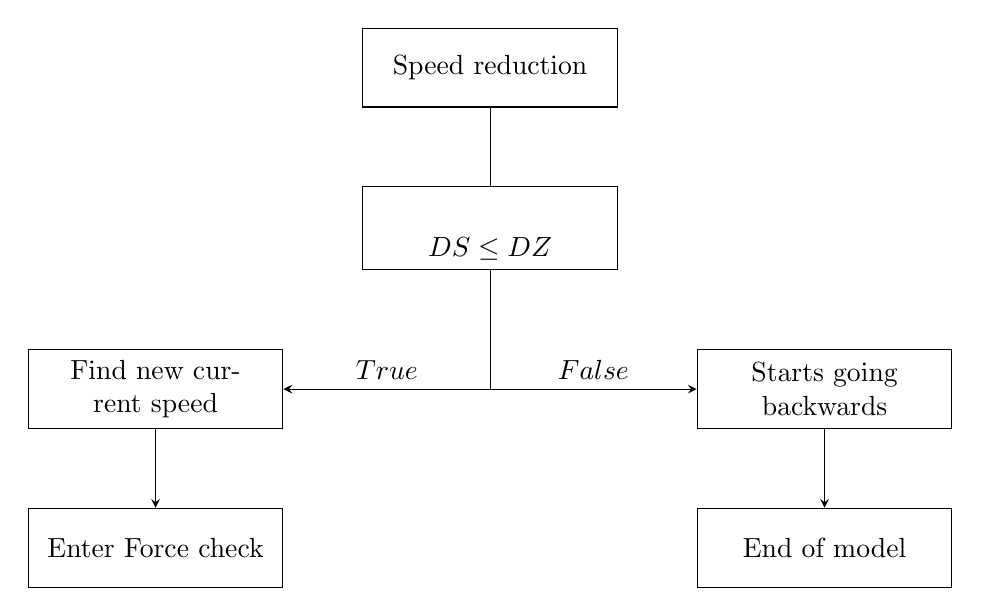
\begin{tikzpicture}
	% draw rectangle node
	\node[draw,
	minimum width=2cm,
	minimum height=1cm,
	text width=3cm,
	text centered] (block1) {
	Speed reduction
	};
	\node[draw,
	minimum width=2cm,
	minimum height=1cm,
	below=of block1,
	text width=3cm,
	text centered] (block2) {
	$$ DS \leq DZ $$
	};
	\node[draw,
	minimum width=2cm,
	minimum height=1cm,
	below left=of block2,
	text width=3cm,
	text centered] (block3) {
	Find new current speed
	};
	\node[draw,
	minimum width=2cm,
	minimum height=1cm,
	below right=of block2,
	text width=3cm,
	text centered] (block4) {
	Starts going backwards
	};
	\node[draw,
	minimum width=2cm,
	minimum height=1cm,
	below=of block3,
	text width=3cm,
	text centered] (block5) {
	Enter Force check
	};
	\node[draw,
	minimum width=2cm,
	minimum height=1cm,
	below=of block4,
	text width=3cm,
	text centered] (block6) {
	End of model
	};
	% Line
	\draw (block1.south) -- ++(block2);
	
	% Arrows
	\draw[-stealth] (block2) |- (block3) node[near end,above]{$True$};
	\draw[-stealth] (block2) |- (block4) node[near end,above]{$False$};
	\draw[-stealth] (block3) edge (block5);
	\draw[-stealth] (block4) edge (block6);
	\end{tikzpicture}

\caption{Speed reduction flowchart diagram.}
\label{fig:SpeedReductionDiagram}
\end{figure}

\subsubsection{Calculating \textbf{\textit{DZ}}}
To be able to compare $DS$ and $DZ$, we first need to calculate $DZ$. Since both the initial and final velocities are known, a formula for displacement using these parameters are used, see formula \ref{eq:D}.
\begin{equation}
\label{eq:D}
D = \frac{(V_0 + V) \cdot t}{2}
\end{equation}

The time $(t)$ is unknown, and it is therefore needed to either solve it or change this part of the formula. By solving the velocity formula for time instead of velocity an new expression for time $(t)$ is acquired. This result in formula \ref{eq:t}:

\begin{equation}
\label{eq:t}
V = V_0 + at \Rightarrow t = \frac{V - V_0}{a}
\end{equation}

Acceleration $(a)$ is needed for both this new expression of time and potentially later for calculation the new current speed. This acceleration can be acquired by using the force formula, and solving it for acceleration:
\begin{equation}
\label{eq:a}
F = ma \Rightarrow a = \frac{F}{m}
\end{equation}

The final formula for $DZ$ is acquired by placing formula \ref{eq:t} into formula \ref{eq:D}, and setting $V = 0$, which leads to formula \ref{eq:DZ}:

\begin{equation}
\label{eq:DZ}
DZ = \frac{- (V_0^2)}{2a}
\end{equation}


\subsubsection{Calculating the new current speed \textit{(V)}}
The velocity squared formula is needed to find the new current speed $(V)$ at the end of the state. Since this step is only occurring if $DZ$ is equal or greater than $DS$ and therefore gives a positive $V$, it is safe to compute the square root of the term $V_0^2 + 2a DS$. This results in the following formula:

\begin{equation}
\label{eq:V}
V^2=V_0^2 + 2a \cdot D \Rightarrow V=\sqrt{V_0^2 + 2 a \cdot DS}
\end{equation}


\subsection{Speed gain}
\begin{figure} [H]
\centering
	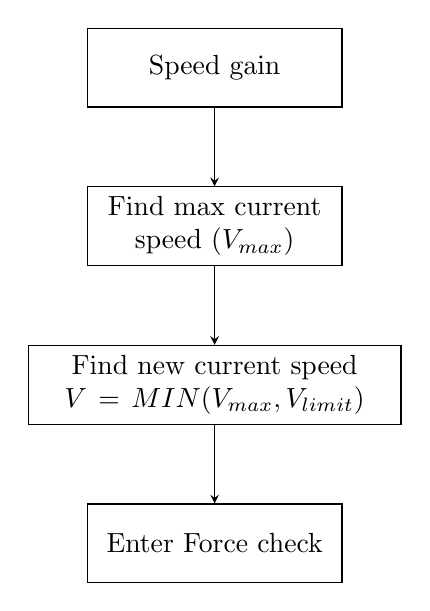
\begin{tikzpicture}
	% draw rectangle node
	\node[draw,
	minimum width=2cm,
	minimum height=1cm,
	text width=3cm,
	text centered] (block1) {
	Speed gain
	};
	\node[draw,
	minimum width=2cm,
	minimum height=1cm,
	below=of block1,
	text width=3cm,
	text centered] (block2) {
	Find max current speed $(V_{max})$
	};
	\node[draw,
	minimum width=2cm,
	minimum height=1cm,
	below=of block2,
	text width=4.5cm,
	text centered] (block3) {
	Find new current speed $V=MIN(V_{max}, V_{limit})$
	};
	\node[draw,
	minimum width=2cm,
	minimum height=1cm,
	below=of block3,
	text width=3cm,
	text centered] (block4) {
	Enter Force check
	};
	
	% Arrows
	\draw[-stealth] (block1) edge (block2);
	\draw[-stealth] (block2) edge (block3);
	\draw[-stealth] (block3) edge (block4);
	\end{tikzpicture}

\caption{Speed gain flowchart diagram}
\label{fig:SpeedGainDiagram}
\end{figure}


Figure \ref{fig:SpeedGainDiagram} gives an overview of the steps in the Speed gain state. The first step is to find the max current speed $(V_{max})$ that is possible. The formula \ref{eq:V} is also used for calculating $V_{max}$. Even if the truck can gain a high speed, it is still limited by road regulations such as speed limits. The second step of the Speed gain state is therefore to set the new current speed $(V)$ to lowest velocity of $V_{max}$ or the speed limit $(V_{limit})$. The new current speed is therefore: 
\begin{equation}
\label{eq:Speed}
V= \text{MIN}(V_{max}, V_{limit})
\end{equation}

\subsection{Gear range}
To make the simulations more realistic a speed range is needed to be put on each gear. This is due to the engine force being a product of the gear ratio. Taking this and the fact that the lower gears have a higher gear ratio into consideration, you would always produce the highest engine force with lower gears. This sounds great in theory, but low gears also produce low speeds and can therefore only be used when the truck is driving in low speeds. Unfortunately there are no “rules” stating what velocity is fitting for each gear.
\par
This type of truck have a max speed of 90km/h and 12 driving gears, these driving gears does not include reverse nor the crawling gears. The 12 driving gears are divided into 8 gears, where 5 to 8 is divided into low (LO) and high (HI) gears. To create the speed ranges, two methods was applied.
\par
The first method is to divide the max speed into 8 sections, then divide the LO and HI gears into two. This creates the following ranges: 

%Table of Gear range 1
\begin{table}[H]
\renewcommand{\arraystretch}{1.15}
\center
\begin{tabular}{| p{0.3\linewidth} | p{0.3\linewidth} | p{0.3\linewidth} |} 

 \hline
 \textbf{Gear} & \multicolumn{2}{|c|}{\textbf{Range [km/h]}} \\
 \hline 
1 & 0 & 11.25 \\
2 & 11.25 & 22.5 \\
3 & 22.5 & 33.75 \\
4 & 33.75 & 45 \\
5LO & 45 & 50.625 \\
5HI & 50.625 & 56.25 \\
6LO & 56.25 & 61.875 \\
6HI & 61.875 & 67.5 \\
7LO & 67.5 & 73.125 \\
7HI & 73.125 & 78.75 \\
8LO & 78.75 & 84.375 \\
8HI & 84.375 & 90 \\
 \hline
\end{tabular}
\caption{Tables of gear range, without overlap, using the first method of dividing.}
\label{tab:gearsM1}
\end{table}

%END of Table of  Gear range 1

The second method is to divide the max speed into 12 sections. This creates the following ranges:

%Table of Gear range 2
\begin{table}[H]
\center
\begin{tabular}{| p{0.3\linewidth} | p{0.3\linewidth} | p{0.3\linewidth} |} 

 \hline
 \textbf{Gear} & \multicolumn{2}{|c|}{\textbf{Range [km/h]}} \\
 \hline 
1 & 0 & 7.5 \\
2 & 7.5 & 15 \\
3 & 15 & 22.5 \\
4 & 22.5 & 30 \\
5LO & 30 & 37.5 \\
5HI & 37.5 & 45 \\
6LO & 45 & 52.5 \\
6HI & 52.5 & 60 \\
7LO & 60 & 67.5 \\
7HI & 67.5 & 75 \\
8LO & 75 & 82.5 \\
8HI & 82.5 & 90 \\
 \hline
\end{tabular}
\caption{Tables of gear range, using the second method of dividing.}
\label{tab:gearsM2}
\end{table}

%END of Table of  Gear range 2

The speed ranges used in the simulation are created by combining the ranges from method one and two, then overlap the range over the neighbouring ranges. This means that gear 2 can be used in the rages for gear 1, 2 and 3. This creates the following ranges:

%Table of Gear range 3
\begin{table}[H]
\center
\begin{tabular}{| p{0.12\linewidth} | p{0.18\linewidth} | p{0.18\linewidth} | p{0.18\linewidth} | p{0.18\linewidth} |} 

 \hline
 \textbf{Gear} & \multicolumn{2}{|c|}{\textbf{Range [km/h]}} & \multicolumn{2}{|c|}{\textbf{Simulation range [km/h]}} \\
 \hline 
1 & 0 	& 11.25 	& 0 		& 22.5 \\
2 & 7.5 	& 22.5 	& 0 		& 33.75 \\
3 & 15 	& 33.75	& 7.5		& 45 \\
4 & 22.5	& 45		& 15		& 50.625 \\
5LO & 30 	& 50.625	& 22.5	& 56.25 \\
5HI & 37.5 & 56.22	& 30		& 61.875 \\
6LO & 45 	& 61.875	& 37.5	& 67.5 \\
6HI & 52.5 & 67.5	& 45		& 73.125 \\
7LO & 60 	& 73.125	& 52.5	& 78.75 \\
7HI & 67.5 & 78.75	& 60		& 84.375 \\
8LO & 75 	& 84.375	& 67.5	& 90 \\
8HI & 82.5 & 90		& 75		& 90 \\
 \hline
\end{tabular}
\caption{Tables of the gear ranges used in the simulations.}
\label{tab:gears}
\end{table}

%END of Table of  Gear range 3


\section {Validation}
\label {validation}
There are mainly two steps of the validation, to validate the variable assumptions taken and then validate the model. It is crucial to validate and potentially tune the variables used for the model to be accurate. The gear ranges from table \ref{tab:gears}, are some of the most important variables to validate. This is due to them having a huge impact on the simulation as well as being essentially guessed. 

After potentially tuning and validating the variables, they can now be used for validating the model. Validating the model is simply done by comparing the result of the model and experiments.

\subsection{Experiments}
When validating the model and its variables it is important to collect data, this can be done through experiments. Many modern trucks have the equipment needed to measure the truck variables such as total mass, $AR$, velocity and engine speed, that can be calculated to engine torque. Environmental variables such as the friction coefficient needs specialized equipment for measuring, while other variables like $Wr$ and gear ratio can to be looked up in spec sheets. 
\par
The experiments can be conducted in several different approaches. Where one is to simply to re-enact the simulations in real life while collecting the needed data. One challenge with performing an experiment like this, is having a secure area where all the environmental variables are known.


\section{Implementation}
\label{implementation}
The models are created by using Python and Excel. All the environments and their variables are listed in an Excel file. This Excel file is then read by a Python script, that uses these listed variables to create the environments for the models. The models and all the results can be found on the online repository ~\citep{repo}.
\par
The Python script that reads the Excel file used several libraries. NumPy ~\citep{numpy} and Pandas ~\citep{pandas} are both used to create and format an array of the environment variables. These packages are used for scientific computing and data analysis. To actually read the data from the Excel file, xlrd 1.2.0 ~\citep{xlrd} is used. Xlrd is a package for reading data and formatting information from Excel files. In addition to these packages, matplotlib~\citep{plt} was used to take the results and format them into graphs and tables. 


\chapter{Results}
\label{results}
This chapter is dedicated to the result of several simulations with different initial velocity, gear ratio and environment for the trucks R580 6x2 and 6x4. There are three environments used, TB\_1, TB\_2 and TB\_3. These environments are all based on Taraldsvikbakken, but under different road conditions. The gradient of the hill is found using the Norwegian Public Roads Administration’s map tool, Vegkart ~\citep{vegkart}.
\par
The results was obtained by using the truck variables in table \ref{tab:usedVariables}, unless specified otherwise. On the result graphs, each gear is named GR followed by the gear number, for example: 5LO is listed as GR5LO. If there are several gears listed, for example “R580\_6x2\_GR5LO\_GR3\_GR4”, it means that the result applies for all the gears listed. 

%Table of variables
\renewcommand{\arraystretch}{1.2}
\begin{table}[H]
\center
\begin{tabular}{|p{0.49\linewidth} | p{0.49\linewidth}|} 

 \hline
\multicolumn{2}{|c|}{\textbf{Truck variables}} \\
 \hline 
m[$kg$] & 40000 \\

AR & \makecell[l]{6x4: 2/6 \\ 6x2: 1/6} \\

DR & 3.42 \\

TE & 0.7 \\

Wr[$m$] & 0.522 \\

ET[$Nm$] & 2950 \\

 \hline
\end{tabular}
\caption{Tables of variables used in simulations}
\label{tab:usedVariables}
\end{table}

%END of Table of variables


\section{Velocities for enviorment TB\_1:}
The environment TB\_1 is the entire hill with a constant friction coefficient of 0.28. This friction coefficient represent normal winter tyres on relatively good winter road conditions, such as dry snow and ice. A similar friction coefficient can also be achieved by sniping the tyres or applying chains on poor road conditions such as wet ice and snow. The following table specifies the variables for TB\_1 :
%Table of TB_1
\renewcommand{\arraystretch}{1.2}
\begin{table}[H]
\center
\begin{tabular}{|p{0.17\linewidth} | p{0.16\linewidth} | p{0.16\linewidth} | p{0.16\linewidth} | p{0.17\linewidth} |} 

 \hline
\multicolumn{5}{|c|}{\textbf{Variables for TB\_1}} \\
 \hline 
Gradient [\%]  & Angle[deg]  & \makecell[l]{Friction\\coefficient} & DS [m]  & $V_{limit}$[km/h]  \\
\hline
8.5 & 4.86 & 0.28 & 150.0 & 60.0 \\
 \hline
\end{tabular}
\caption{Tables of variables for enviorment TB\_1}
\label{tab:TB1}
\end{table}
%END of Table of TB_1

\subsection{Truck R580 6x2}
The R580 6x2 managed to ascent TB\_1 for all the chosen initial velocities while constantly maintaining one gear. The amount of gears that was used to successfully ascent differs depending on the initial velocity, as seen in the following figure:

%TB_1 6x2
\begin{figure}[H]
\includegraphics[width=\textwidth, height=0.37\textheight]{photo/freeBodyDiagram.png}
\caption{Velocities for: enviorment TB\_1, R580 6x2 with different gear and initial velocity.}
\label{fig:TB1_6x2}
\end{figure}

The R580 6x2 successfully ascended TB\_1, for four out of five of the initial velocities during the FG sim. The result of the successful ascensions can be seen on the following figure:
\begin{figure}[H]
\includegraphics[width=\textwidth, height=0.45\textheight]{photo/freeBodyDiagram.png}
\caption{Velocities for: enviorment TB\_1, R580 6x2 with different gear and initial velocity. Gear down one gear at 75m.}
\label{fig:TB1_6x2_GR}
\end{figure}

The R580 6x2 failed to ascend TB\_1 with an initial velocity of 40km/h during the FG sim, regardless of starting gear. The following figure shows the result of the failed ascensions with the eligible gears for the initial velocity:
\begin{figure}[H]
\includegraphics[width=\textwidth, height=0.45\textheight]{photo/freeBodyDiagram.png}
\caption{Graph of velocities for a R580 6x2 with different gear and $V_0 = 40$. Gear down one gear after 75m.}
\label{fig:TB1_6x2_GR_40}
\end{figure}

\subsection{Truck R580 6x4}
% TB_1 6x4
Due to the amount of plots and repeating plot colours, the plots for figure \ref{fig:TB1_6x4} and \ref{fig:TB1_6x4_GR} are also labelled with initial velocity (V0). 
\par
The R580 6x4 was able to ascent TB\_1 for all the chosen initial velocities while constantly maintaining one gear. For certain gears, the truck was even able to gain speed as shown in the following figure:
\begin{figure}[H]
\includegraphics[width=\textwidth, height=0.37\textheight]{photo/freeBodyDiagram.png}
\caption{Velocities for: enviorment TB\_1, R580 6x4 with different gear and initial velocity}
\label{fig:TB1_6x4}
\end{figure}

The R580 6x4 managed to ascent TB\_1 for all initial velocities during the FG sim. For certain gears the R580 6x4 was even able to accelerate as seen in the following graph:
\begin{figure}[H]
\includegraphics[width=\textwidth, height=0.37\textheight]{photo/freeBodyDiagram.png}
\caption{Velocities for: enviorment TB\_1, R580 6x4 with different gear and initial velocity. Gear down one gear at 75m}
\label{fig:TB1_6x4_GR}
\end{figure}



\section{Velocities for enviorment TB\_2:}
Environment TB\_2 divides the hill into five uneven sections with different friction coefficients. These friction coefficients represent a particularly slippery day with poor road conditions. The following table specifies the variables for TB\_2 from bottom to top of the hill:
%Table of TB_2
\renewcommand{\arraystretch}{1.2}
\begin{table}[H]
\center
\begin{tabular}{|p{0.17\linewidth} | p{0.16\linewidth} | p{0.16\linewidth} | p{0.16\linewidth} | p{0.17\linewidth} |} 

 \hline
\multicolumn{5}{|c|}{\textbf{Variables for TB\_2}} \\
 \hline 
Gradient [\%]  & Angle[deg]  & \makecell[l]{Friction\\coefficient} & DS [m]  & $V_{limit}$[km/h]  \\
\hline
8.5 & 4.86 & 0.25 & 25.0 & 60.0 \\
8.5 & 4.86 & 0.15 & 40.0 & 60.0 \\
8.5 & 4.86 & 0.10 & 30.0 & 60.0 \\
8.5 & 4.86 & 0.11 & 30.0 & 60.0 \\
8.5 & 4.86 & 0.16 & 25.0 & 60.0 \\
 \hline
\end{tabular}
\caption{Tables of variables for enviorment TB\_2}
\label{tab:TB2}
\end{table}
%END of Table of TB_2

\subsection{Truck R580 6x2}
%TB_2 6x2
The R580 6x2 successfully ascended TB\_2, for two out of five of the initial velocities during the BD sim. The result of the successful ascensions can be seen on the following figure:
\begin{figure}[H]
\includegraphics[width=\textwidth, height=0.37\textheight]{photo/freeBodyDiagram.png}
\caption{Graph of velocities for a R580 6x2 with different gear and initial velocity}
\label{fig:TB2_6x2}
\end{figure}

The R580 6x2 failed to ascend TB\_2 with an initial velocity of 50km/h during the BD sim regardless of having an end velocity of 14.89km/h. This end velocity is outside of the gear range for all eligible starting gears, resulting in a failed ascension. The following figure shows the result of the failed ascensions with the eligible gears for the initial velocity:
\begin{figure}[H]
\includegraphics[width=\textwidth, height=0.45\textheight]{photo/freeBodyDiagram.png}
\caption{Velocities for: enviorment TB\_2, R580 6x2 with different gear and $V_0 = 50$.}
\label{fig:TB2_6x2_50}
\end{figure}

The R580 6x2 failed to ascend TB\_2 with an initial velocity of 45km/h during the BD sim, regardless of starting gear. The following figure shows the result of the failed ascensions with the eligible gears for the initial velocity:
\begin{figure}[H]
\includegraphics[width=\textwidth, height=0.37\textheight]{photo/freeBodyDiagram.png}
\caption{Velocities for: enviorment TB\_2, R580 6x2 with different gear and $V_0 = 45$.}
\label{fig:TB2_6x2_45}
\end{figure}

The R580 6x2 failed to ascend TB\_2 with an initial velocity of 40km/h during the BD sim, regardless of starting gear. The following figure shows the result of the failed ascensions with the eligible gears for the initial velocity:
\begin{figure}[H]
\includegraphics[width=\textwidth, height=0.37\textheight]{photo/freeBodyDiagram.png}
\caption{Velocities for: enviorment TB\_2, R580 6x2 with different gear and $V_0 = 40$.}
\label{fig:TB2_6x2_40}
\end{figure}
 
% GR
The R580 6x2 successfully ascended TB\_2, for three out of five of the initial velocities during the FG sim. The result of the successful ascensions can be seen on the following figure:
\begin{figure}[H]
\includegraphics[width=\textwidth, height=0.45\textheight]{photo/freeBodyDiagram.png}
\caption{Graph of velocities for a R580 6x2 with different gear and initial velocity. They gear down one gear after 75m}
\label{fig:TB26x2GR}
\end{figure}

The R580 6x2 failed to ascend TB\_2 with an initial velocity of 45km/h during the FG sim, regardless of starting gear. The following figure shows the result of the failed ascensions with the eligible gears for the initial velocity:
\begin{figure}[H]
\includegraphics[width=\textwidth, height=0.37\textheight]{photo/freeBodyDiagram.png}
\caption{Velocities for: enviorment TB\_2, R580 6x2 with different gear and $V_0 = 45$. Gear down one gear at 75m.}
\label{fig:TB2_6x2_45}
\end{figure}

The R580 6x2 failed to ascend TB\_2 with an initial velocity of 40km/h during the FG sim, regardless of starting gear. The following figure shows the result of the failed ascensions with the eligible gears for the initial velocity:
\begin{figure}[H]
\includegraphics[width=\textwidth, height=0.37\textheight]{photo/freeBodyDiagram.png}
\caption{Velocities for: enviorment TB\_2, R580 6x2 with different gear and $V_0 = 40$. Gear down one gear at 75m.}
\label{fig:TB2_6x2_40}
\end{figure}


\subsection{Truck R580 6x4}
% TB_2 6x4
The R580 6x4 managed to ascent TB\_2 for all initial velocities during the BD sim. The results can be seen in the following graph:
\begin{figure}[H]
\includegraphics[width=\textwidth, height=0.45\textheight]{photo/freeBodyDiagram.png}
\caption{Graph of velocities for a R580 6x4 with different gear and initial velocity}
\label{fig:TB26x4}
\end{figure}

The R580 6x4 managed to ascent TB\_2 for all initial velocities during the FG sim. The results can be seen in the following graph:
\begin{figure}[H]
\includegraphics[width=\textwidth, height=0.45\textheight]{photo/freeBodyDiagram.png}
\caption{Graph of velocities for a R580 6x4 with different gear and initial velocity. They gear down one gear after 75m}
\label{fig:TB26x4GR}
\end{figure}


\section{Velocities for enviorment TB\_3:}
The environment TB\_3 is the hill divided into ten even sections with different friction coefficient. These friction coefficients indicates poor road conditions at the bottom that gradually improves during the ascension. The following table specifies the variables for TB\_3 from bottom to top of the hill:
%Table of TB_3
\renewcommand{\arraystretch}{1.2}
\begin{table}[H]
\center
\begin{tabular}{|p{0.17\linewidth} | p{0.16\linewidth} | p{0.16\linewidth} | p{0.16\linewidth} | p{0.17\linewidth} |} 

 \hline
\multicolumn{5}{|c|}{\textbf{Variables for TB\_3}} \\
 \hline 
Gradient [\%]  & Angle[deg]  & \makecell[l]{Friction\\coefficient} & DS [m]  & $V_{limit}$[km/h]  \\
\hline
8.5 & 4.86 & 0.17 & 15.0 & 60.0 \\
8.5 & 4.86 & 0.20 & 15.0 & 60.0 \\
8.5 & 4.86 & 0.21 & 15.0 & 60.0 \\
8.5 & 4.86 & 0.23 & 15.0 & 60.0 \\
8.5 & 4.86 & 0.22 & 15.0 & 60.0 \\
8.5 & 4.86 & 0.24 & 15.0 & 60.0 \\
8.5 & 4.86 & 0.28 & 15.0 & 60.0 \\
8.5 & 4.86 & 0.28 & 15.0 & 60.0 \\
8.5 & 4.86 & 0.28 & 15.0 & 60.0 \\
8.5 & 4.86 & 0.28 & 15.0 & 60.0 \\
 \hline
\end{tabular}
\caption{Tables of variables for enviorment TB\_3}
\label{tab:TB3}
\end{table}
%END of Table of TB_3

\subsection{Truck R580 6x2}
The R580 6x2 successfully ascended TB\_3, for four out of five of the initial velocities during the BD sim. The result of the successful ascensions can be seen on the following figure:
%TB_3 6x2
\begin{figure}[H]
\includegraphics[width=\textwidth, height=0.38\textheight]{photo/freeBodyDiagram.png}
\caption{Graph of velocities for a R580 6x2 with different gear and initial velocity}
\label{fig:TB36x2}
\end{figure}

The R580 6x2 failed to ascend TB\_3 with an initial velocity of 40km/h during the BD sim, regardless of starting gear. The following figure shows the result of the failed ascensions with the eligible gears for the initial velocity:
\begin{figure}[H]
\includegraphics[width=\textwidth, height=0.45\textheight]{photo/freeBodyDiagram.png}
\caption{Velocities for: enviorment TB\_3, R580 6x2 with different gear and $V_0 = 40$.}
\label{fig:TB3_6x2_40}
\end{figure}

The R580 6x2 successfully ascended TB\_3, for four out of five of the initial velocities during the FG sim. The result of the successful ascensions can be seen on the following figure:
\begin{figure}[H]
\includegraphics[width=\textwidth, height=0.37\textheight]{photo/freeBodyDiagram.png}
\caption{Graph of velocities for a R580 6x2 with different gear and initial velocity. They gear down one gear after 75m}
\label{fig:TB36x2GR}
\end{figure}

The R580 6x2 failed to ascend TB\_3 with an initial velocity of 40km/h during the FG sim, regardless of starting gear. The following figure shows the result of the failed ascensions with the eligible gears for the initial velocity:
\begin{figure}[H]
\includegraphics[width=\textwidth, height=0.37\textheight]{photo/freeBodyDiagram.png}
\caption{Velocities for: enviorment TB\_3, R580 6x2 with different gear and $V_0 = 40$. Gear down one gear at 75m.}
\label{fig:TB3_6x2_40}
\end{figure}


\subsection{Truck R580 6x4}
% TB_3 6x4
The R580 6x4 managed to ascent TB\_3 for all initial velocities during the BD sim. The results can be seen in the following graph:
\begin{figure}[H]
\includegraphics[width=\textwidth, height=0.45\textheight]{photo/freeBodyDiagram.png}
\caption{Graph of velocities for a R580 6x4 with different gear and initial velocity}
\label{fig:TB36x4}
\end{figure}

The R580 6x4 managed to ascent TB\_3 for all initial velocities during the FG sim. The results can be seen in the following graph:
\begin{figure}[H]
\includegraphics[width=\textwidth, height=0.45\textheight]{photo/freeBodyDiagram.png}
\caption{Graph of velocities for a R580 6x4 with different gear and initial velocity. They gear down one gear after 75m}
\label{fig:TB36x4GR}
\end{figure}

\chapter{Discussion}
This chapter comments and discusses the thesis and its results from the \nameref{results} chapter. Before looking at the results, it is important to note that the actual speed limit in Taraldsvikbakken is 50km/h. For the sake of seeing if the initial velocity have an impact on the result, the $V_{limit}$ is set to 60km/h during the simulation.
\par 
Python is used for this thesis because it is easy to use and handles both text and numerical parameters elegantly. Being able to use the matplotlib package was also favouring the usage of Python, this is because Matplotlib is extremely easy to use and helpful for formatting the results into graphs and tables. The runtime of the script is relatively short, where it uses most of its time to create and save the huge amount of graphs and tables.

\section{Environment}
The environment have the most impact on the ascension, but unfortunately it is something that cannot often be altered or changed. The only variable that can be changed is the friction coefficient between the road and the tyres. The impact the friction coefficient have can clearly be seen by comparing the results of the same truck and simulation on the different environments. 
\par
As expected an environment with lower friction coefficients makes the truck have a higher deacceleration. There are several things that can be done to rise the friction coefficients, such as putting on chains or siping of truck tyres. Unfortunately these changes works as a precautions which means they require to be applied before the truck starts ascending or even before it starts driving.

\section{Truck comparison}
There are certain statements that can be concluded by comparing the results of the 6x2 and 6x4. A 6x4 truck have a greater chance of successfully ascending a hill than a 6x2 truck. Additionally a 6x4 truck have a higher velocity after ascending the hill. This can clearly be seen by comparing the 6x2 with the 6x4 figures of the same simulation and environment. 
\par
In certain cases the 6x4 was even able to accelerate parts of the ascending as seen in figure \ref{fig:TB1_6x4}, \ref{fig:TB1_6x4_GR}, \ref{fig:TB36x4} and \ref{fig:TB36x4GR}. During these cases it is clear to see that certain gears are more beneficial than others. This is connected to the formulas used for finding the forward force $F_F$. Since the 6x4 have a higher $AR$ than the 6x2, the $F_f$ is therefore higher. This gives a greater chance of the $F_F$ being limited by the $F_e$, instead of the $F_f$. Whenever the $F_F$ is limited by the $F_e$ the gear that is being used can drastically change the result, as seen in the figures mentioned above.

\section{Failed ascensions}
There are many reasons why a truck might fail an ascension. All these reasons for failing the ascension leads to one main problem: loss of velocity. With the earlier set limits, such as eligible starting gear and speed limit these reasons can be limited to a few. 
\par
According to the results, one of the main reasons for the failed ascensions are the trucks not having a high enough initial velocity. This is because a truck with a low initial velocity, uses a longer time to ascent a hill. When the truck deaccelerate over time, the more time it spends ascending the more velocity it loses. This turns into a vicious circle where the truck eventually ends up failing the ascension.
\par
When comparing the results from figure \ref{fig:TB1_6x2} and \ref{fig:TB1_6x2_GR}, another reason for a failed ascension can be seen. During the FG sim the 6x2 is not able to ascent TB\_1 with an initial velocity of 40km/h, unlike the BD sim. The reason for the failed ascension is therefore the gear change. With an already low velocity changing gear is catastrophic. This is because the truck have no $F_F$ during the gear change, making the 6x2 rapidly deaccelerate. Due to the low velocity after the gear change, the 6x2 is not able to ascent TB\_1. This can be seen in figure \ref{fig:TB1_6x2_GR_40}.
\par

\section{Gear change}
The FG sim performs worse when comparing the end velocity between the BD sim and the FG sim results. For the amount of starting gears that results in a successful ascension the FG sim performs better. This is due to the trucks in general losing velocity over time, that results in the velocity going out of range for the gear used. When the gear change occurs the lower limit of the range goes down.
\par
When comparing figure \ref{fig:TB2_6x2} and \ref{fig:TB26x2GR}, it can be seen that during the FG sim the truck was able to ascent TB\_2 with an initial velocity of 50km/h unlike the BD sim. When studying figure \ref{fig:TB2_6x2_50} it is clear that the failed ascension during the BD sim is due to the end velocity being out of range for the testing gears. This suggests that even if gearing down lowers the velocity, it might be needed for the truck to be able to ascent. 
\par
The fact that gearing down can both save and fail an ascension, confirms the previously mentioned hypothesis concerning the importance of how the driver is driving. An experienced driver might known or have a hunch of when it is beneficial to change gear and therefore have a greater chance of ascending the hill. By further studying these make it or brake it cases some correlation can be seen. 
\par
As the rate of deceleration increases the chance of a gear change being beneficial increases. This applies only and only if the truck still have a decent current velocity. A gear change cannot save a rapidly deaccelerating truck with an already low velocity. As mentioned earlier the friction coefficient heavily affects the deacceleration of the truck. This means that if the environment has a low friction coefficient the chances of a gear change being beneficial increases. 


\chapter{Conclusion}
This thesis have researched the possibility of creating a simulation, and looked at the different aspects of a simplified simulation. It is definitely possible to create a realistic simulation, and a simplified model is useful. The results from this simplified simulation makes sense, and are similar to our predicted outcome based on statements and experiences from professionals. Unfortunately no physical experiments where conducted during the thesis so the accuracy cannot be proven, but it is believed that this simplified simulation could be rather accurate after tuning the parameters. 
\par
The effect of different weight distribution, initial velocity and friction coefficient can clearly be seen from the results. Where more weight on the driver axles, higher initial velocity and higher friction coefficient helps increasing the chances of ascending a hill. Another important aspect of ascending the hill, is how the driver is driving. Changing gear at the wrong time can have catastrophic consequences, while changing gear on the correct time can save the ascension attempt. 
\par
A simple simulation can be as useful as a complex simulation, especially when it comes to calculating the friction coefficient. There are many variables needed that can quickly change over time when calculating a friction coefficient in a complex simulation. It is therefore needed to take these inaccuracies into consideration. This take a lot of computation time for something that might not have a notable difference to the accuracy. A bit more complex simulation might have a more accurate calculation of the engine force and slightly different handling of the friction coefficients. These changes, does not need to make the simulation much more complex but could potentially make it more accurate.

\section{Future work}
The most important next step for this research would be to have experiments validating the variables and simulation. If needed the simulations should be made more complex, researching where the inaccuracies might originate from. After experiments and potentially tuning the simulation, a more “smart” gear shift simulation should be added. This type of simulation would be more of a realistic driving, and might potentially help say when someone needs to change gears for optimal hill ascension. 
\par



% Include the bibliography
\bibliographystyle{apalike}
\bibliography{bibl}

\backmatter
\end{document}7